\section{Architecture}
In \autoref{arch}, a broad overview of the architecture of the application is given. 

    \begin{figure}[H]
		\centering
		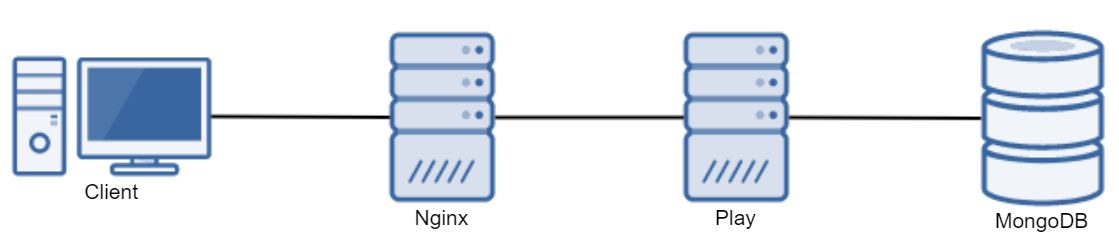
\includegraphics[width=1.0\textwidth]{images/Architecture.png}
		\caption{Overview of the architecture of Uber for Bikes}
		\label{arch}
	\end{figure}
	
An instance of the application has several virtual machines running so that each could be placed on different hardware. 

For our webserver we have written the main component in Scala. Scala is functional programming language supporting high scalability. To write not everything from scratch, we used the Play Framework. 

For our project we used for our database MongoDB with ReactiveMongo. ReactiveMongo is a Scala driver that provides fully non-blocking and asynchronous I/O operations. ReactiveMongo is designed to avoid any kind of blocking request. Every operation return immediately, freeing the running thread and resuming execution when it is over.

In the frond-end AngularJS and Bootstrap is used for providing a nice user interface. The UI serves a simple purpose: Renting and unrenting bikes. The main view of the UI is a Google Maps view. It is currently set to the location of Groningen, but could eventually be used to show the region where the user resides.
In our project we use an external third party service. The service of Google is needed to convert a textural representation of a location into the corresponding geographical representation of the GPS system. This conversion is done via the Google Maps API.


\subsection{Docker swarm}

Explain the docker swarm